The fixed-template estimator applied to the 17 individual exposures gives pooled 2382 and 2600 shifts relative to 2374 of $-41.9\pm16.4$ and $-45.5\pm15.0\,\mathrm{m\,s^{-1}}$. Applying the same estimator to the combined spectrum gives $-42.8$ and $-39.6\,\mathrm{m\,s^{-1}}$. These are compatible representations of the same observations, not independent confirmations. They are also different estimators from the joint fits in which all gas parameters are re-optimized. The original exposure analysis finds no clear excess heterogeneity or difference between the nine 2018 and eight later exposures under its conditional covariance model.

The same-transition comparison removes the atomic reference entirely. In the initial per-exposure calculation, the lower-index minus upper-index order contrast is $-60.25\pm16.72\,\mathrm{m\,s^{-1}}$ for 2600, compared with $-10.53\pm21.87\,\mathrm{m\,s^{-1}}$ for 2382. The two traces separately retain the 2600 pattern, and deleting any single exposure gives means between approximately $-70.1$ and $-52.0\,\mathrm{m\,s^{-1}}$. The diagnostic is therefore not dominated by one exposure or one trace. The barycentric velocity and detector position are nearly collinear in these observations, preventing their simple regressions from locating the mechanism.

We next fit all exposures jointly with the Gaussian and centred positive-mixture response families defined in Sec.~\ref{sec:methods}. Each family has matched comparisons with and without a single order-contrast parameter. This jointly shared response estimator is slightly different from independently fitting each exposure. The completed comparisons are shown in Table~\ref{tab:order_models} and Fig.~\ref{fig:order_models}.

\begin{table}[htbp]
\centering
\caption{Native-pixel order-response controls. The order contrast is the lower-index minus higher-index order velocity for the same transition, distinct from the cross-transition descriptor $D$. G denotes the Gaussian response; A denotes the specified positive, zero-centroid asymmetric family. Subscripts indicate whether a free order contrast is added. Errors are local, conditional on the fixed gas template and diagonal extraction errors. $\Delta Q$ compares models within the indicated response family, not different transitions.}
\label{tab:order_models}
\small
\begin{tabular}{llrrr}
\toprule
Transition & Response & $Q$ & Order contrast ($\mathrm{m\,s^{-1}}$) & $\Delta Q$ \\
\midrule
2600 & G$_0$ & 41636.411 & 0 (fixed) & --- \\
2600 & G$_1$ & 41622.198 & $-62.75\pm16.66$ & 14.212 \\
2600 & A$_0$ & 41630.900 & 0 (fixed) & --- \\
2600 & A$_1$ & 41620.042 & $-58.64\pm18.65$ & 10.858 \\
2382 & G$_0$ & 39994.136 & 0 (fixed) & --- \\
2382 & G$_1$ & 39993.889 & $-11.03\pm22.18$ & 0.247 \\
2382 & A$_0$ & 39994.062 & 0 (fixed) & --- \\
2382 & A$_1$ & 39993.787 & $-13.48\pm26.35$ & 0.275 \\
\bottomrule
\end{tabular}
\end{table}

The specified asymmetric family does not remove the 2600 contrast. Relative to G$_1$, two shape parameters reduce $Q$ by only 2.16. Forcing a zero order contrast in A$_0$ drives one shape parameter to its bound. The asymmetric fit has nominal $Q/(N-k)\simeq1.34$ for 2600 and 1.29 for 2382, so even the extended response does not supply an adequate complete noise-and-profile description. Conditional objective profiles explicitly re-optimize the remaining parameters at 13 order offsets from $-120$ to $+120\,\mathrm{m\,s^{-1}}$. They confirm the local displacement preference while exposing shape boundaries; they do not supply a calibrated discovery probability. The shape parameterization is not generally twice continuously differentiable at its Gaussian limit, providing another reason to avoid an automatic Wilks interpretation.

\begin{figure}[htbp]
\centering
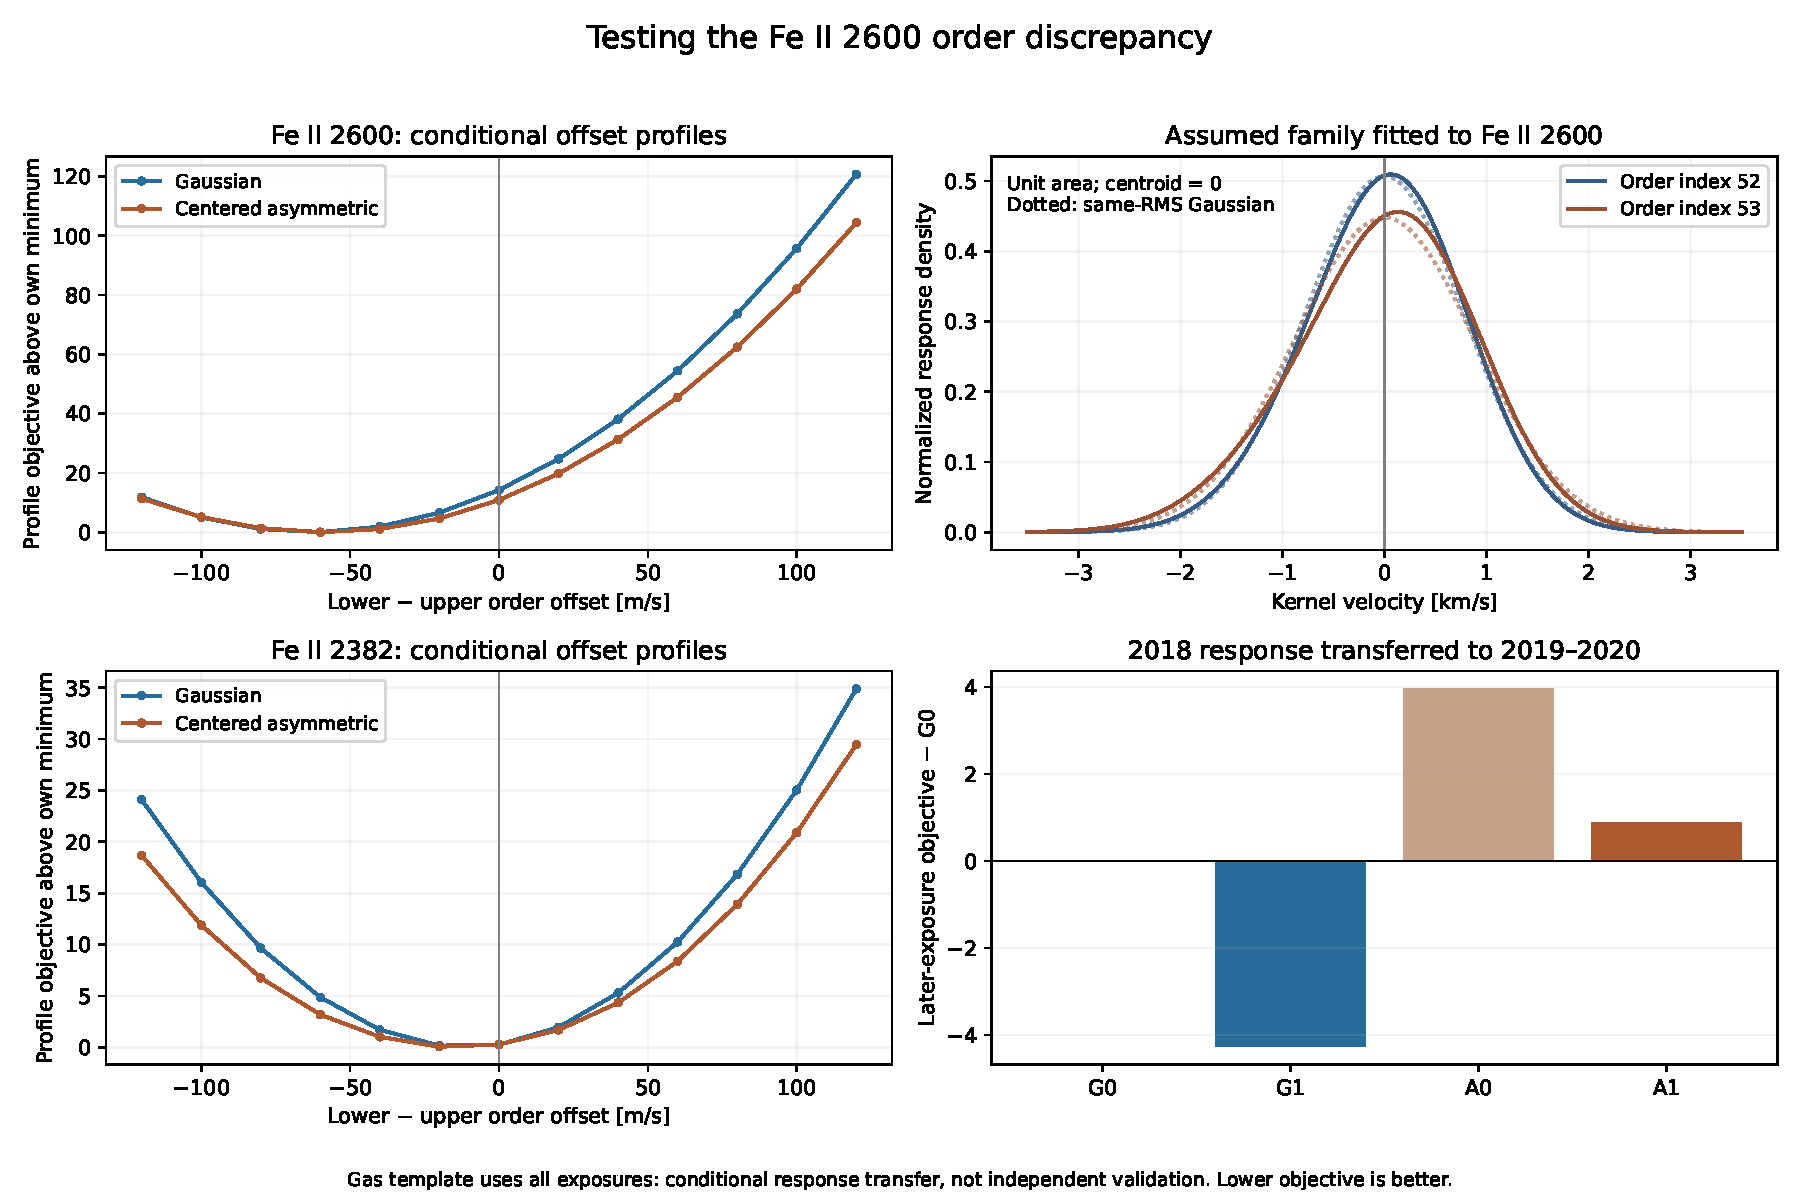
\includegraphics[width=.99\textwidth]{../experiments/highz_feasibility_2026-09-20/results/order_response/order_response_models.pdf}
\caption{Tests of the specified centred response family using actual native pixels. The order-contrast profiles re-optimize nuisance parameters at fixed contrast. The response-family illustration does not represent an independently measured LSF. The later-exposure comparison transfers response parameters learned from 2018, while the gas template remains shared with the full data set; it is therefore a conditional transfer diagnostic.}
\label{fig:order_models}
\end{figure}

In that transfer diagnostic, the Gaussian-plus-contrast model improves the later-exposure objective by 4.27 relative to the Gaussian zero-contrast model. The asymmetric-plus-contrast model is worse than Gaussian-plus-contrast by 5.15. This does not establish a transferable benefit from the extra shape parameters. An instrumental response that genuinely changes across epochs remains possible, and the shared combined-spectrum gas template prevents a fully independent predictive interpretation.

The orders also have different sampling, masks and signal-to-noise weights. A further mask control retains a native pixel only when its entire wavelength bin is covered by the other order's originally valid bins; selection uses wavelength geometry and existing quality masks, not new residual clipping. It retains 62,154 of 62,404 relevant pixels. The resulting 2600 contrast is $-58.65\pm16.75\,\mathrm{m\,s^{-1}}$, and the 2382 contrast is $-15.45\pm21.98\,\mathrm{m\,s^{-1}}$. Missing coverage alone, under this particular control, does not remove the pattern. Sampling and weighting still differ, so a shared imperfect gas template could produce different apparent velocities without a pure calibration offset.

Independent calibration remains unresolved. The released science headers identify the same \texttt{espdr/2.2.3}, SINGLEHR, $2\times1$ mode and LFC/FP wavelength products. For two representative science frames, current default archive master associations instead return THAR/FP wavelength products. Their association status does not establish reproduction of the released LFC solution. We locate historical raw LFC candidates and preserve their headers and association trees, but the checked public links do not yield uniquely matched historical LFC masters or independently measured response kernels. The 2024 response study used 2023 calibration data \citep{Schmidt2024LSF}; its method motivates this investigation, while its measured kernels cannot simply be assigned to the 2018--2020 science exposures. The bounded controls therefore locate a robust conditional order inconsistency without identifying its unique cause or measuring an intrinsic atomic change.
